\documentclass[11pt,a4paper,final]{article}

\usepackage[utf8]{inputenc}
\usepackage[spanish]{babel}
\usepackage[left=2.5cm,right=2.5cm,top=2.5cm,bottom=2.5cm]{geometry}

\usepackage[colorlinks = true, linkcolor = blue]{hyperref}
\usepackage{listings}
\usepackage{graphicx}
\usepackage{subfig}
\usepackage{url}


\author{Pablo Rodríguez Guillén (Representante): 32733455Q \\
		José Márquez Doblas: 46074763J}
\title{\textbf{Problema de las Jarras de Agua en CLIPS}}
\date{10 de mayo de 2019}

\setlength \parindent{0em}
\setlength \parskip{1em}

\begin{document}

\nocite{*}

\maketitle
\tableofcontents
\newpage

\section{Enunciado del Problema}
El objetivo de este trabajo es la implementación de las técnicas de búsqueda primero en profundidad y primero en anchura para solucionar un problema típico de Inteligencia Artificial. El problema de las jarras de agua. El planteamiento del problema es el siguiente:

Disponemos de dos jarras de agua, una de 4 litros de capacidad y otra de 3 litros de capacidad. Inicialmente están ambas vacías. El estado objetivo es que la jarra de 4 litros de capacidad contenga dos litros de agua, independientemente el contenido de la otra, sabiendo que en ninguna de las jarras hay una señal de volumen distinta de su capacidad. Para conseguir este objetivo, podemos realizar las siguientes acciones:

\begin{enumerate}
	\item Llenar la jarra de 4 litros completamente (para ello, la jarra de 4 litros no debe estar completamente llena).
	\item Llenar la jarra de 3 litros completamente (para ello, la jarra de 3 litros no debe estar completamente llena).
	\item Vaciar la jarra de 4 litros (para ello, la jarra debe contener algo de liquido).
	\item Vaciar la jarra de 3 litros (para ello, la jarra debe contener algo de liquido).
	\item Verter el contenido de la jarra de 4 litros en la jarra de 3 litros (para ello, la jarra de 4 litros debe contener algo de liquido y la de 3 litros no estar completamente llena).
	\item Verter el contenido de la jarra de 3 litros en la jarra de 4 litros (para ello, la jarra de 3 litros debe contener algo de liquido y la de 4 litros no estar completamente llena).
\end{enumerate}

Identificar y representar los hechos necesarios para resolver el problema en clips mediante las dos técnicas de búsqueda comentadas anteriormente. Ha de controlarse también que no haya nodos repetidos.

\newpage

\section{Estrategia empleada}
\subsection{Representación de la información}
Para representar la información del problema hemos utilizado hechos no ordenados, utilizando una plantilla \emph{node} a través del constructor \emph{deffacts}. La plantilla cuenta con tres atributos: 

\begin{itemize}
	\item \textbf{\emph{multisolt jars}}: durante todo el programa contendrá un hecho ordenado con los siguientes 4 sibolos: \emph{j3 x j4 y} siendo \emph{x} e \emph{y} los valores que representan el contenido de la jarra de cuatro litros y de tres litros. Estos valores van a oscilar entre cero y cuatro, dado que la lógica implementada en las reglas no lo permite de otro modo.
	\item \textbf{\emph{slot father}}: contiene un hecho del tipo \emph{FACT-ADRESS SYMBOL}, es decir, la dirección de memoria de otro hecho. En este caso, será un hecho ordenado \emph{node} que apuntará al nodo padre del nodo en cuestión. Hay un símbolo permitido \emph{none}, para poder representar a la raíz del árbol del problema, que no tiene nodo padre.
	\item \textbf{\emph{slot level}}: contiene un número entero que representa el nivel del profundidad del nodo en el árbol. La profundidad de un nodo es la profunidad del padre más uno. La profundidad del nodo raíz es 0.
\end{itemize}

\subsection{Análisis de diseño e implementación}
En los siguientes apartados se detalla la estrategia concreta seguida para los métodos de búsqueda \hyperref[anchura]{primero en anchura} y \hyperref[profundidad]{primero en profundidad}. A un nivel más general hemos implementado reglas que se podrían dividir en dos grupos.

\begin{itemize}
	\item Reglas de las operaciones permitidas por el enunciado para generar nuevos estados:
	
	\begin{itemize}
		\item \textbf{Llenado de jarras:} Se permite siempre que la jarra a llenar no esté llena de antemano.
		\item \textbf{Vaciado de jarras:} Se permite siempre que la jarra a vaciar no esté vacía de antemano.
		\item \textbf{Vertido de una jarra en otra:} Existen dos versiones de la regla para cada jarra. Esto es porque  el comportamiento de la regla varía si al verter una jarra en otra se derrama el contenido, lo cual no se permite en el problema. Para solucionar esto planteamos dos soluciones, utilizar funciones procedurales de tipo \emph{if} o implementar dos reglas. Optamos por la segunda opción ya que se nos recomendaba usar el menor número de funciones procedurales posibles.
	\end{itemize}
	
	\item Reglas para controlar el flujo del programa:
	
	\begin{itemize}
		\item \textbf{\emph{initial}:} Se ejecuta siempre al principio, ya que el único hecho en la base de hechos al inicio del programa es el \emph{initial-fact}. Afirma el hecho correspondiente al nodo raíz del árbol del problema.
		\item \textbf{\emph{removeTwins}:} Por cada nodo, se generan todos los hijos posibles. Esto causa que estados que ya hayan aparecido anteriormente durante la ejecución del programa se vuelvan a crear. Para evitar esto, la regla \emph{removeTwins} tiene una prioridad muy alta y sus antecedentes se comprueban cada vez que se genera un nuevo nodo. Si el nuevo nodo es uno repetido, se activa la regla y se elimina el nodo.
		\item \textbf{\emph{finalResult}:} Al igual que \emph{removeTwins} tiene una prioridad muy alta, sus antecedentes comprueban si el nodo en cuestión tiene la jarra de cuatro litros con dos litros. Si se activa, el programa muestra el contenido de la base de hechos con el comando \emph{(facts)} y finaliza.
	\end{itemize}
\end{itemize}

\subsubsection{Búsqueda primero en anchura} \label{anchura}
Para que el programa haga una búsqueda primero en anchura, hay que asegurar que no se incremente el nivel con el que se generan los nuevos nodos, hasta que no se hayan generado todos los nodos de un mismo nivel. 

Para controlar esto, hemos definido un hecho \emph{globalLevel n} donde \emph{n} es el nivel de los padres que están generando nuevos nodos en un momento determinado de la ejecución de nuestro programa. Estos nuevos nodos, como es lógico, incrementan su nivel en una unidad. Para asegurarnos de que esto es así, todas las reglas que generan nuevos nodos del archivo \emph{JarrasAnchura.clp} tienen un antecedente que comprueba que el nivel del nodo que activa la función es igual al que alberga \emph{globalLevel}.

Cuando todos los nodos de un mismo nivel han generado todos sus hijos posibles (recordamos que cada vez que se genera un nuevo nodo se pueden activar las reglas de \emph{removeTwins} y \emph{finalResult}) activando las reglas que generan nuevos nodos, se activa una función de menor prioridad que solo hemos implementado en la búsqueda primero en anchura que simplemente incrementa \emph{globalLevel} en una unidad, lo que permite que los estados de un nivel mayor, puedan activar reglas. Esta función es \emph{increaseLevel}.

\subsubsection{Búsqueda primero en profundidad} \label{profundidad} 
La implementación de este método de búsqueda es mucho más directa en CLIPS ya que este, es un sistema basado en reglas que trabaja con la información más reciente. De manera que los hechos más recientes se colocan al final de la tabla de la base de hechos y las reglas comprueban sus antecedentes con hechos de abajo a arriba, en cuanto a posición en la base de hechos se refiere.

De manera que al eliminar el antecedente que exigía, en la búsqueda primero en anchura, que los nodos fueran del mismo nivel, el programa genere nuevos hijos con los nodos de mayor profundidad, ya que estos siempre van a ser los más recientes generados. Por la misma razón no es necesario incluir la regla \emph{increaseLevel}.

\newpage

\section{Manual de usuario}
La ejecución de los programas es muy sencilla, simplemente debemos abrir \emph{CLIPS} en el directorio \emph{code} del fichero \emph{.zip} extraído y ejecutar los siguientes comandos:

\begin{itemize}
	\item Para la búsqueda primero en anchura:
\end{itemize}

\begin{lstlisting}
	(load JarrasAnchura.clp)
	(reset)
	(run)
\end{lstlisting}

\begin{itemize}
	\item Para la búsqueda primero en profundidad:
\end{itemize}

\begin{lstlisting}
	(load JarrasProfundidad.clp)
	(reset)
	(run)
\end{lstlisting}

\begin{figure}[ht]
	\centering
	\subfloat[Búsqueda Primero en Anchura]{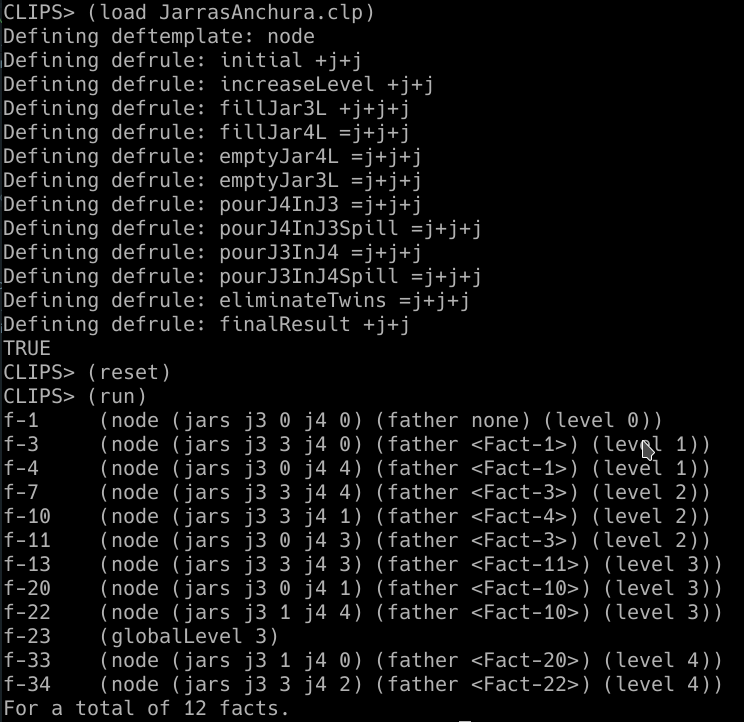
\includegraphics[width=0.44\textwidth]{Anchura.png}}
	\qquad
	\subfloat[Búsqueda Primero en Profundidad]{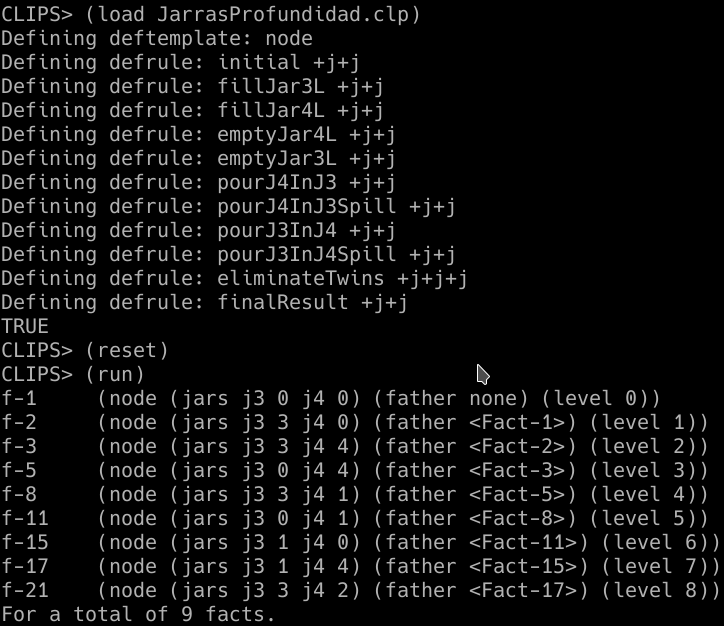
\includegraphics[width=0.44\textwidth]{Profundidad.png}}
\end{figure}

\newpage

\section{Roles en el desarrollo}
La coordinación entre nosotros a lo largo del desarrollo del proyecto ha sido muy buena. La fase inicial se hizo de forma conjunta. Consistió en el diseño general de reglas que íbamos a necesitar y la codificación de la búsqueda primero en anchura. Esto se debe a que vimos que la búsqueda primero en profundidad requería de menos condiciones. Durante esta fase inicial 

Nos enfocamos en implementar la búsqueda y en que funcionara. Cuando llegamos a ese punto dividimos totalmente el trabajo. José Márquez se ha dedicado a la mejora del código inicial: eliminación de hechos irrelevantes que no aportaban lo que pensamos en un inicio durante la fase de diseño y adición de comentarios. Además, se ha encargado de la implementación de la búsqueda en profundidad, que dado el comportamiento de CLIPS y partiendo del código de la búsqueda primero en anchura resultó más o menos sencillo.

Por otro lado, Pablo Rodríguez Guillén se ha encargado de la elaboración de la memoria del proyecto al completo.

\clearpage

\addcontentsline{toc}{section}{Referencias}
\bibliography{bibliography}
\bibliographystyle{unsrt}
	
\end{document}